\chapter{随机变量及其分布}
\section{随机变量}
\dfn{随机变量}{
    设随机试验的样本空间为$S$,称定义在$S$上的实值单值函数$X=X(\omega)$为\vocab{随机变量}.\\
    亦即
    \[X:\omega\mapsto x_i \in \RR\,\, \mathrm{i.e.}\,\,S\rightarrow\RR\]
}
实际上,$\Pr(X=a)$是$A=\{\omega|X(\omega)=a\}$的简记.
\section{离散型随机变量及其分布}
设$X$是一个随机变量,如果$X$的所有可能取值为有限个或可列无限多个,则称$X$为\vocab{离散型随机变量}.
\dfn{离散型随机变量分布律}{
    设$X$是一个离散型随机变量,如果
    \[\Pr(X=x_k)=p_k,k=1,2,\cdots\]
    则称$p_k$为$X$的\vocab{分布律}或\vocab{概率分布},亦称\vocab{概率质量函数}(PMF). 记为$f_X(x)$.
}
就是高中所学之分布列.
\subsection{常用离散分布}
\subsubsection{两点分布}
\dfn{两点分布}{
    设$X$的分布律为
    \begin{align}
        \Pr(X=k)=\begin{cases}
                     p,   & k=x_1 \\
                     1-p, & k=x_2
                 \end{cases}
    \end{align}

    其中$0<p<1$,则称$X$服从以$p$为参数的\vocab{两点分布}.
}
若$X$服从$x_1 = 1,x_2 = 0$处参数为$p$的两点分布,则称其服从参数为$p$的\vocab{0-1分布}.
\subsubsection{二项分布}
\leftnote[1cm]{当$n=1$时,二项分布退化为0-1分布.}
\dfn{二项分布}{
    设$X$的分布律为
    \begin{equation}
        \Pr(X=k)=\binom{n}{k}p^k(1-p)^{n-k},\,\,k=0,1,\cdots,n
    \end{equation}
    其中$n$为正整数,$0<p<1$,则称$X$服从参数为$n,p$的\vocab{二项分布},记为$X\sim B(n,p)$.
}
\leftnote{$\sim$记号就是\textbf{服从}的意思}
二项概率总存在一个最大值$M$ s.t. \((n+1)p-1\leq M<(n+1)p\).
\subsubsection{Poisson分布}
\dfn{Poisson分布}{
    设$X$的分布律为
    \begin{equation}
        \Pr(X=k)=\frac{\lambda^k}{k!}e^{-\lambda},\,\,k=0,1,\cdots
    \end{equation}
    其中$\lambda>0$,则称$X$服从参数为$\lambda$的\vocab{Poisson分布},记为$X\sim P(\lambda)$.
}
因为$e^x=1+\sum_{n=1}^{\infty}\frac{x^n}{n!}$,将$x$换为$\lambda$可得泊松分布的概率和为1.
\section{累积分布函数}
\subsection{随机变量的分布函数}
\dfn{随机变量CDF}{
    设$X$是一个随机变量,对任意实数$x$,定义
    \[F(x)=\Pr(X\leq x)\in [0,1]\]
    称$F(x)$为$X$的\vocab{累积分布函数}(CDF). 有时记作$F_X(x)$或$X\sim F(x)$.
}
分布函数$F(x)$的值就表示$X$落在区间$(-\infty,x]$的概率.
\subsubsection{性质}
\begin{enumerate}
    \item \textit{单调非减性}: $x_1<x_2\Rightarrow F(x_1)\leq F(x_2)$
    \item $F(-\infty) = \lim_{x\rightarrow -\infty}F(x) = 0,\,\,F(+\infty) = \lim_{x\rightarrow +\infty}F(x) = 1$.
    \item \textit{右连续性}: $\lim_{x\rightarrow x_0^+}F(x) = F(x_0)$
\end{enumerate}
具有上述性质的函数一定是某个随机变量的CDF.
\clearpage
\subsection{离散型随机变量的分布函数}
在上述基础上,对于离散型随机变量$X$有CDF:
\[F(x) = \Pr(X\leq X) = \sum_{x_i\leq x}\Pr(X=x_i)\]

\begin{figure}[h]
    \centering
    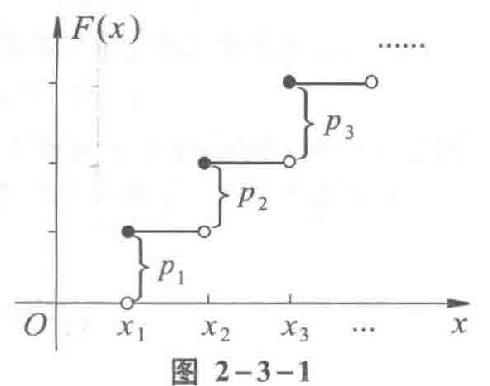
\includegraphics[scale=.5]{cdf_discrete}
    \caption{阶梯型CDF}
\end{figure}
$F(x)$是一个\vocab{阶梯型函数},在点$x_i$处的跃度为$\Pr(X=x)$.
可以看出阶梯型函数符合CDF之性质:总是右连续的;而作为一个分段函数来说,其各段区间总是左闭右开的.
\nt{
    考题中由CDF反推分布列可以根据每一个左侧端点得到对应的随机变量$x_i$.\\
    计算分布列时,有公式$\Pr{a\leq X< b} = F(b) - F(a)$.
}
随机变量$X$的CDF为阶梯型函数$\Leftrightarrow$ $X$是离散型随机变量.
\section{连续型随机变量及其概率密度}
\dfn{PDF}{
    设$X$是一个随机变量,如果存在非负可积函数$f(x)$,使对任意实数$x$有
    \begin{equation}
        F(x) = \Pr{X\leq x} = \int_{-\infty}^xf(t)\dd t
    \end{equation}
    则称$X$为\vocab{连续型随机变量},$f(x)$为$X$的\vocab{概率密度函数}(PDF).
}
立即可以得到PDF的性质
\begin{enumerate}
    \item $f(x)\geq 0$;
    \item $\int_{-\infty}^{+\infty}f(x)\dd x = 1$.
    \item $F'(x) = f(x)$. 若f(x)在x处连续
\end{enumerate}
\nt{
    若某个随机变量的CDF可以写成PDF积分函数的形式,则称其为连续型随机变量.
}
\pf{证明    X取任一特值的概率为$0$}{
    \begin{align*}
        \mbox{考虑极限}
        \Pr{X=a} & =\lim_{\Delta x \leftarrow 0^+}\Pr{a-\Delta x \le X \leq a}   \\
        \mbox{对RHS积分,有}                                                          \\
        \Pr{X=a} & =\lim_{\Delta x \leftarrow 0^+}\int_{a-\Delta x}^{a}f(x)\dd x \\
                 & =0.
    \end{align*}
}
由上面的证明我们可以知道以下的性质
\begin{equation}
    \Pr{a< X< b } = F(b ) - F(a ) = \int_{a }^{b }f(x )\dd x.
\end{equation}
无论X两侧端点开闭都成立.
\subsection{常用连续型分布}
\subsubsection{均匀分布}
\dfn{均匀分布}{
    设$X$的概率密度为
    \begin{equation}
        f(x)=\begin{cases}
            \frac{1}{b-a}, & a<x<b \\
            0,             & else
        \end{cases}
    \end{equation}

    其中$a<b$,则称$X$服从参数为$a,b$的\vocab{均匀分布},记为$X\sim U(a,b)$.
}
\leftnote[-1cm]{U stands for Uniform}
设$[a,b]$之间的任意子区间为$[c,d]$,由上式可得$\Pr{c<X<d}=\int_{c }^{d }\frac{1}{b-a}\dd x = \frac{d-c}{b-a}$.\\因而我们可以得到
\cor{均匀分布的CDF}{
    \begin{equation}
        F(x) = \begin{cases}
            0,               & x < a     \\
            \frac{x-a}{b-a}, & a\leq x<b \\
            1,               & x\geq b
        \end{cases}
    \end{equation}
}
\subsubsection{指数分布}
\dfn{指数分布}{
    若随机变量$X$的概率密度为
    \begin{equation}
        f(x)=\begin{cases}
            \lambda e^{-\lambda x}, & x>0     \\
            0,                      & x\leq 0
        \end{cases}, \lambda > 0
    \end{equation}
    则称X服从参数为$\lambda$ 的\vocab{指数分布},记为$X\sim E(\lambda)$.
}
积分得
\cor{指数分布的CDF}{
    \begin{equation}
        F(x)=\begin{cases}
            1-e^{-\lambda x}, & x>0     \\
            0,                & x\leq 0
        \end{cases}
    \end{equation}
}
\subsubsection{正态分布}
\dfn{正态分布}{
    若随机变量$X$的概率密度为
    \begin{equation}
        f(x)=\frac{1}{\sqrt{2\pi}\sigma}e^{-\frac{(x-\mu)^2}{2\sigma^2}},\,\,-\infty<x<+\infty
    \end{equation}
    其中$\mu,\sigma(\sigma>0)$为常数,则称$X$服从参数为$\mu,\sigma^2$的\vocab{正态分布},记为$X\sim N(\mu,\sigma^2)$.
}
\qs{Poisson积分}{
    \textbf{不使用Wallis公式},求Poisson积分:\\
    \begin{equation*}
        \int_{-\infty}^{+\infty}e^{-t^2}\dd t
    \end{equation*}
}

\sol{
    \textit{分析法}
    \begin{align}
        \text{要求原式,不妨先求其平方,亦即}                                                                                                                                            \nonumber \\
        \left(\int_{-\infty}^{+\infty}e^{-t^2}\dd t\right)^2                              & = \int_{-\infty}^{+\infty}e^{-x^2}\dd x\int_{-\infty}^{+\infty}e^{-y^2}\dd y \nonumber  \\
        \text{化为累次积分有}                                                                                                                                                    \nonumber \\
                                                                                          & = \int_{-\infty}^{+\infty}\int_{-\infty}^{+\infty}e^{-(x^2+y^2)}\dd x\dd y.  \nonumber  \\
        \text{相当于在平面内求此积分,化为极坐标有}                                                                                                                                         \nonumber \\
        \int_{-\infty}^{+\infty}\int_{-\infty}^{+\infty}e^{-\rho^2}\rho\dd \rho\dd \theta & = \int_{0}^{2\pi}\dd \theta\int_{0}^{+\infty}e^{-\rho^2}\rho\dd \rho       \nonumber    \\
                                                                                          & = \pi                                                                         \nonumber \\
        \tf \int_{-\infty}^{+\infty}e^{-t^2}\dd t                                         & = \sqrt{\pi}.
    \end{align}
}
通过证明Poisson积分,我们可以得到正态分布的PDF重要性质
\begin{equation}
    \int_{-\infty}^{+\infty}\frac{1}{\sqrt{2\pi}\sigma}e^{-\frac{(x-\mu)^2}{2\sigma^2}}\dd x = 1
\end{equation}
\newpage
\textbf{图形特征}
\begin{figure}[h]
    \centering
    \includesvg[scale=.75]{Normal_Distribution_PDF}
    \caption{PDF}
\end{figure}
\leftnote[5cm]{$\sigma$越小,方差越大,曲线中峰越陡}
\begin{enumerate}
    \item $\mu$确定曲线位置, $\sigma$确定曲线中峰的陡峭程度
    \item 密度曲线关于$x=\mu$对称
    \item 密度曲线在$x=\mu$处有最大值$\frac{1}{\sqrt{2\pi}\sigma}$
    \item 密度曲线在$x=\mu\pm\sigma$处有拐点且以$x$轴为渐近线
\end{enumerate}
当$\mu=0,\sigma=1$时,称为\vocab{标准正态分布},记为$X\sim N(0,1)$,PDF用$\phi(x )$表示,CDF用$\Phi(x )$表示.
\begin{align}
    \phi(x ) = \frac{1}{\sqrt{2\pi}}e^{-\frac{x^2}{2}} &  & \Phi(x ) = \int_{-\infty}^{x}\phi(t)\dd t
\end{align}
\thm{}{
    设$X\sim N(\mu,\sigma^2)$,则$Y= \frac{X-\mu}{\sigma}\sim N(0,1)$.\\
    计算$\Pr{Y\leq x}$时,可转化为计算$\Pr{X\leq \mu + \sigma x}$,计算此时的$\Phi(x)$即得证.
}
这说明任何一个一般的正态分布都可以通过\textbf{线性变换}转化为标准正态分布.
因此X的分布函数也可以写成
\[F(x) = \Phi\left(\frac{x-\mu}{\sigma}\right)\]
\[\Pr{a<X<b}= \Pr{\frac{a-\mu}{\sigma}<Y<\frac{b-\mu}{\sigma}} = \Phi\left(\frac{b-\mu}{\sigma}\right) - \Phi\left(\frac{a-\mu}{\sigma}\right)\]